\documentclass[aspectratio=169,10pt]{beamer}
\usepackage[utf8]{inputenc}
\usepackage[T1]{fontenc}
\usepackage{lmodern}
\usepackage{graphicx}
\usepackage{microtype}
\usepackage{ragged2e}
\usepackage{booktabs,tabularx,array,multirow}
\usepackage{amsmath,amssymb}
\usepackage{tikz}
\usetikzlibrary{arrows.meta,positioning,shapes.geometric,fit,calc}
\usepackage{pgfgantt}
\usepackage{xcolor}
\usepackage{hyperref}
\usepackage{plan4ari_beamer}
\hypersetup{colorlinks=true,linkcolor=planblue,urlcolor=planblue,citecolor=planblue}
\setlength{\tabcolsep}{4pt}
\renewcommand{\arraystretch}{1.15}
\emergencystretch=1em

\title[Plan4ARI]{Plan4ARI\\\large Planning for Artificial Robotic Intelligence and Beyond}
\subtitle{Integrated architecture for trustworthy industrial autonomy}
\author{Nicola Pedrocchi}
\institute{COMAU \and CNR}
\date{March, 19th 2026}

\begin{document}
\begin{frame}
  \titlepage\
\end{frame}
\begin{frame}{Agenda}

\tableofcontents

\end{frame}


\section{Motivation and Vision}

\begin{frame}{Project at a Glance}

\begin{columns}[T,totalwidth=\textwidth]
\column{0.58\textwidth}
\begin{itemize}
  \item \textbf{Acronym:} Plan4ARI.\@
  \item \textbf{Title:} Planning for Artificial Robotic Intelligence and Beyond.
  \item \textbf{Duration:} 48 months.
  \item \textbf{Area:} Advanced Manufacturing.
  \item \textbf{PI:} Nicola Pedrocchi.
  \item \textbf{Host Institution:} COMAU.\@
  \item \textbf{Research Organization:} CNR.\@
\end{itemize}
\column{0.40\textwidth}
\begin{block}{Strategic goal}
Develop an \textbf{Artificial Robotic Intelligence (ARI)} stack that makes industrial robots easier to program, safer to deploy, and more adaptive in dynamic human-robot environments.
\end{block}
\end{columns}

\end{frame}


\begin{frame}{Why Plan4ARI?}

\begin{itemize}
  \item Industrial robots are powerful but still constrained by \textbf{specialized programming}, lengthy engineering cycles, and limited adaptation to changing environments.
  \item The proposal argues that recent progress in \textbf{large language models, deliberative AI, deep sensing, adaptive motion planning, and neural control} can now be systematically integrated.
  \item The central thesis is that cognitive capability must be distributed across \textbf{all controller layers}:\@user interaction, task planning, motion planning, and real-time execution.
  \item The result is not a generic AGI claim, but a practical \textbf{Industry~5.0 architecture} for trustworthy robotic autonomy.
\end{itemize}
%\refs{Source:\@proposal sections ``From AGI to ARI'' and Abstract.}

\end{frame}


\begin{frame}{From AGI to ARI}

\begin{columns}[T,totalwidth=\textwidth]
\column{0.48\textwidth}
\begin{block}{AGI perspective}
The proposal frames AGI as the long-term ambition of systems able to understand, learn, and reason across tasks.
\end{block}
\begin{block}{Industrial constraint}
Manufacturing does not need unconstrained general intelligence; it needs \textbf{robust, safe, and verifiable intelligence} embedded in robot workflows.
\end{block}
\column{0.48\textwidth}
\begin{block}{ARI perspective}
Plan4ARI defines \textbf{Artificial Robotic Intelligence} as the coordinated integration of:
\begin{itemize}
  \item natural language programming,
  \item task allocation and scheduling,
  \item scene understanding and safe motion planning,
  \item adaptive real-time motion control.
\end{itemize}
\end{block}
\end{columns}
%\refs{Source:\@proposal section ``From Artificial Generic Intelligence (AGI) to Artificial Robotic Intelligence (ARI)''.}

\end{frame}


\begin{frame}{Four Levels of Robotic Intelligence}

\begin{enumerate}
  \item \textbf{Programming intelligence:} the user describes the task instead of coding it.
  \item \textbf{Task intelligence:} the robot allocates and schedules actions across humans and other robots in the scene.
  \item \textbf{Motion intelligence:} the robot plans safe movement under contextual constraints.
  \item \textbf{Execution intelligence:} the controller adapts online to scene evolution and disturbances.
\end{enumerate}
\begin{alertblock}{Implication}
Plan4ARI is built as a layered cognitive stack, not as a single AI module bolted onto a conventional robot.
\end{alertblock}
%\refs{Source:\@proposal description of the four intelligence levels.}

\end{frame}


\begin{frame}{Reference Industrial Scenario}

\begin{itemize}
  \item A \textbf{high-payload mobile manipulator} performs welding operations inside a large boat or ship structure.
  \item The environment is \textbf{unstructured, harmful, and dynamically evolving}; references are weak and many operations are defined on site.
  \item A human operator supervises multiple robots and interacts with the system in \textbf{natural language}.
  \item The system must support virtual preview, error refinement, safe execution, and notification when unexpected conditions arise.
\end{itemize}
\begin{block}{Why this matters}
The scenario is not science fiction:\@the proposal argues that most building blocks already exist, but must be turned into a \textbf{new integrated controller architecture}. 
\end{block}
%\refs{Source:\@proposal section ``The Plan4ARI architecture and the COMAU controller~-~Context''.}

\end{frame}


\begin{frame}{Industrial Pain Points Addressed}

\small
\begin{tabularx}{\textwidth}{>{\bfseries}p{0.20\textwidth} X X}
\toprule
Layer & Current limitation & Plan4ARI response \\
\midrule
Programming & Process experts depend on robot specialists and low-code flows remain complex and suboptimal & Natural-language-based generation of verified flowcharts \\
Task planning & Plans are hard to verify, brittle under uncertainty, and weakly optimized & KB-driven PDDL, formal checks, BT/STNU and MCTS optimization \\
Motion planning & Traditional planners struggle with dynamic scenes, human presence and runtime adaptation & Sensor fusion, informed sampling, safety-aware replanning, MPC micro-interpolation \\
Control & Industrial controllers are difficult to tune and cope poorly with uncertainty and elasticity & Prescribed-performance neural control and knowledge reuse \\
HRI adoption & Trust, workload and acceptance limit deployment in real factories & Subjective and objective trustworthiness assessment integrated in the loop \\
\bottomrule
\end{tabularx}
%\refs{Source:\@proposal objectives and module descriptions.}

\end{frame}


\begin{frame}{Consortium and Positioning}

\begin{columns}[T,totalwidth=\textwidth]
\column{0.48\textwidth}
\begin{block}{COMAU}
Industrial automation and robotics leader, providing the host platform, controller access, laboratories, and targeted demonstrators.
\end{block}
\begin{block}{CNR-STIIMA}
Manufacturing systems, industrial robotics, controls, mechatronics, digital methods, and technology transfer.
\end{block}
\column{0.48\textwidth}
\begin{block}{Strategic fit}
The project combines \textbf{industrial integration capability} with \textbf{scientific depth} across planning, robotics, control, sensing and human factors.
\end{block}
\end{columns}
%\refs{Source:\@proposal sections ``Host Institution'' and ``Affiliation Institution and Research Organization''.}

\end{frame}


\section{Architecture and Technical Concept}

\begin{frame}{Conceptual Architecture:\@Two-IPC Design}

\centering
\begin{tikzpicture}[
  x=1cm,y=1cm,>=Latex,
  every node/.style={align=center,font=\scriptsize},
  ipcbox/.style={draw,rounded corners,fill=white,minimum height=0.58cm,inner sep=2pt},
  openitem/.style={ipcbox,text width=3.55cm,minimum width=3.75cm},
  coreitem/.style={ipcbox,text width=3.10cm,minimum width=3.30cm},
  sideitem/.style={draw,rounded corners,fill=green!8,text width=2.05cm,minimum width=2.25cm,minimum height=1cm,inner sep=2pt}
]
  \node[draw,rounded corners,fill=blue!8,minimum width=4.35cm,minimum height=4.85cm] (open) at (0,0) {};
  \node[font=\footnotesize\bfseries,text=planblue] at (0,2.05) {Open IPC};
  \node[openitem] at (0,1.4) {MI.RA/Dexter low-code interface / dispatcher};
  \node[openitem] at (0,0.66) {Natural language $\rightarrow$ knowledge base / PDDL / BT};
  \node[openitem] at (0,-0.1) {Sensing, registration, segmentation};
  \node[openitem] at (0,-0.9) {Offline / online motion planning};
  \node[openitem] at (0,-1.6) {Digital twin and execution monitor};

  \node[draw,rounded corners,fill=orange!10,minimum width=4.00cm,minimum height=4.85cm] (core) at (5.55,0) {};
  \node[font=\footnotesize\bfseries,text=planorange] at (5.55,2.05) {Core IPC};
  \node[coreitem] at (5.55,1.20) {Hard real-time safety rules};
  \node[coreitem] at (5.55,0.40) {MPC micro-interpolator};
  \node[coreitem] at (5.55,-0.40) {Neural motion controller};
  \node[coreitem] at (5.55,-1.20) {Robot / drive interface};

  \draw[->,thick] (2.25,0.35) -- node[above,sloped,font=\tiny,text width=1.75cm]{trajectory stream / references} (3.45,0.70);
  \draw[<-,thick] (2.25,-0.35) -- node[below,sloped,font=\tiny,text width=2.05cm]{state / safety / execution feedback} (3.45,-0.70);

  \node[sideitem] at (-3.50,1.45) {Human operator\\natural language};
  \node[sideitem] at (-3.50,-0.90) {Cell, PLC, sensors, ROS2};
  \draw[->,thick] (-2.35,1.45) -- (-2.20,1.45);
  \draw[->,thick] (-2.35,-0.90) -- (-2.20,-0.90);

  \node[sideitem] at (9.10,-1.20) {Robot axes / actuators};
  \draw[->,thick] (7.60,-1.20) -- (7.95,-1.20);
\end{tikzpicture}
\vspace{0.05em}
\begin{block}{Interpretation}
The Open IPC hosts cognition, world modelling and planning. The Core IPC preserves deterministic execution, safety enforcement and high-rate control.
\end{block}
%\refs{Source:\@proposal Figure~1 and architecture description.}

\end{frame}


\begin{frame}{Architecture Rationale}

\begin{itemize}
  \item The \textbf{Open IPC} acts as the bridge between the robot controller and the external world:\@user interaction, PLCs, sensors, ROS2, digital twin, and asynchronous planning.
  \item The \textbf{Core IPC} concentrates hard-real-time functions:\@safety, micro-interpolation, and high-rate motion control.
  \item This split is essential because the proposal separates \textbf{non-real-time cognitive functions} from \textbf{deterministic control execution}.
  \item The architecture therefore enables innovation while preserving safety-critical behaviour.
\end{itemize}
%\refs{Source:\@proposal architecture narrative following Figure~1.}

\end{frame}


\begin{frame}{Technical Workflow from User to Robot}

\centering
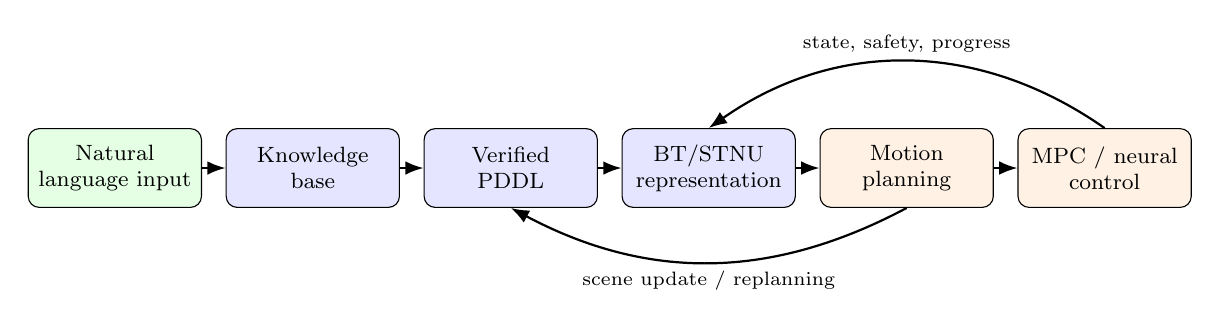
\begin{tikzpicture}[node distance=0.3cm, >=Latex, every node/.style={align=center}]
  \footnotesize
  \node[draw,rounded corners,fill=green!10,minimum width=2.2cm,minimum height=1cm] (u) {Natural\\language input};
  \node[draw,rounded corners,fill=blue!10,minimum width=2.2cm,minimum height=1cm,right=of u] (kb) {Knowledge\\base};
  \node[draw,rounded corners,fill=blue!10,minimum width=2.2cm,minimum height=1cm,right=of kb] (pddl) {Verified\\PDDL};
  \node[draw,rounded corners,fill=blue!10,minimum width=2.2cm,minimum height=1cm,right=of pddl] (bt) {BT/STNU\\representation};
  \node[draw,rounded corners,fill=orange!10,minimum width=2.2cm,minimum height=1cm,right=of bt] (mp) {Motion\\planning};
  \node[draw,rounded corners,fill=orange!10,minimum width=2.2cm,minimum height=1cm,right=of mp] (ctrl) {MPC / neural\\control};
  \draw[->,thick] (u) -- (kb);
  \draw[->,thick] (kb) -- (pddl);
  \draw[->,thick] (pddl) -- (bt);
  \draw[->,thick] (bt) -- (mp);
  \draw[->,thick] (mp) -- (ctrl);
  \draw[->,thick,bend right=35] (ctrl.north) to node[above,font=\scriptsize]{state, safety, progress} (bt.north);
  \draw[->,thick,bend left=28] (mp.south) to node[below,font=\scriptsize]{scene update / replanning} (pddl.south);
\end{tikzpicture}
\begin{block}{Key point}
Plan4ARI links all abstraction levels:\@symbolic planning, geometric planning, and control are coupled through explicit feedback and execution monitoring.
\end{block}
%\refs{Source:\@proposal architecture, low-code module, and motion planning module.}

\end{frame}


\begin{frame}{Project Modules}

\centering
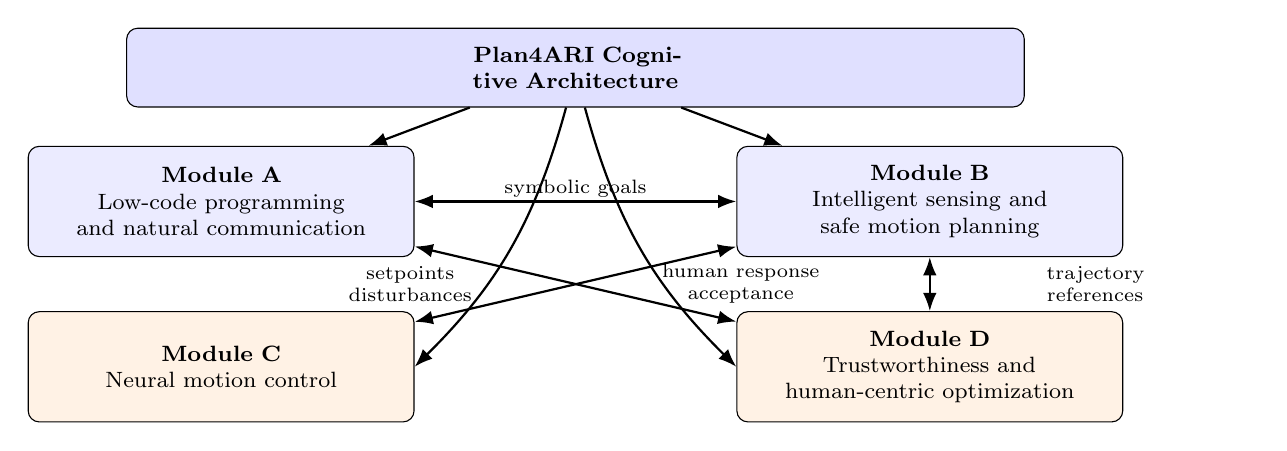
\begin{tikzpicture}[
    x=1cm,y=1cm,>=Latex,
    every node/.style={align=center, text width=4.10cm},
    module/.style={draw,rounded corners,align=center,text width=4.10cm},
    flowlabel/.style={font=\scriptsize,inner sep=1pt}
  ]
  \footnotesize
  \node[draw,rounded corners,fill=blue!12,minimum width=11.4cm,minimum height=1cm] (ari) at (0,2.6) {\textbf{Plan4ARI Cognitive Architecture}};
  \node[draw,rounded corners,fill=blue!8,minimum width=4.9cm,minimum height=1.4cm] (m1) at (-4.5,0.9) {\textbf{Module A}\\Low-code programming and natural communication};
  \node[draw,rounded corners,fill=blue!8,minimum width=4.9cm,minimum height=1.4cm] (m2) at (4.5,0.9) {\textbf{Module B}\\Intelligent sensing and safe motion planning};
  \node[draw,rounded corners,fill=orange!10,minimum width=4.9cm,minimum height=1.4cm] (m3) at (-4.5,-1.2) {\textbf{Module C}\\Neural motion control};
  \node[draw,rounded corners,fill=orange!10,minimum width=4.9cm,minimum height=1.4cm] (m4) at (4.5,-1.2) {\textbf{Module D}\\Trustworthiness and human-centric optimization};
  \draw[->,thick] (ari) -- (m1);
  \draw[->,thick] (ari) -- (m2);
  \draw[->,thick] (ari) edge[bend left=15] (m3.east);
  \draw[->,thick] (ari) edge[bend right=15]  (m4.west);
  \draw[<->,thick] (m1) -- node[above,flowlabel]{symbolic goals} (m2);
  \draw[<->,thick] (m2) -- node[right,flowlabel]{trajectory \\ references} (m4);
  \draw[<->,thick] (m2) -- node[left,flowlabel]{setpoints \\ disturbances} (m3);
  \draw[<->,thick] (m4) -- node[right,flowlabel]{human response\\ acceptance} (m1);
\end{tikzpicture}
\begin{block}{Meaning}
The proposal does not define independent work packages only; it defines a \textbf{functional decomposition of cognition} where outputs from one module directly condition the others.
\end{block}
%\refs{Source:\@proposal Figure~2 and module descriptions.}

\end{frame}


\begin{frame}{Open IPC Responsibilities}

\small
\begin{itemize}
  \item MI.RA/Dexter acts as \textbf{dispatcher} and \textbf{execution monitor} in deliberative-AI terms.
  \item It supports a model-driven, low-code representation where atomic software functionalities are composed into process pipelines.
  \item It hosts scene registration, semantic segmentation, and motion planning modules, and interfaces with ROS2.
  \item It virtualizes operations for the user, enabling preview, validation and monitoring.
  \item It is also the natural insertion point for future AI copilots for process-flow generation.
\end{itemize}
%\refs{Source:\@proposal architecture description of MI.RA/Dexter and Open IPC.}

\end{frame}


\begin{frame}{Core IPC Responsibilities}

\small
\begin{itemize}
  \item Runs the \textbf{real-time motion controller} and a high-rate motion planner or micro-interpolator.
  \item Enforces safety rules and deterministic execution constraints.
  \item Receives streamed references from Open IPC and turns them into real-time setpoints.
  \item Hosts \textbf{Model Predictive Control} for micro-interpolation.
  \item Hosts the \textbf{neural controller} with prescribed-performance design, enabling faster tuning and better tracking in changing conditions.
\end{itemize}
%\refs{Source:\@proposal architecture description and list of Plan4ARI-specific innovations.}

\end{frame}


\begin{frame}{Compliance and Trustworthiness by Design}

\begin{itemize}
  \item The proposal explicitly states that Plan4ARI will be developed in compliance with the \textbf{EU AI Act}, emphasizing safety, transparency, data protection and fundamental rights.
  \item At operational level, human tracking, sensing and decision support are framed with \textbf{GDPR-style mitigation principles}:\@anonymization, online-only processing where possible, and ethics checks.
  \item At control level, collaboration is tied to \textbf{ISO/TS 15066}-style safety reasoning and to trustworthiness metrics developed in Module~D.
\end{itemize}
\begin{alertblock}{Takeaway}
This is not just a performance-driven robotics project; it is a \textbf{trustworthy AI robotics architecture}. 
\end{alertblock}
%\refs{Source:\@proposal architecture section, motion planning section, and barriers/mitigation section.}

\end{frame}


\section{Scientific Module A: Low-Code Programming and Natural Communication}

\begin{frame}{Module A~-~Objective and Positioning}

\begin{itemize}
  \item The objective is to let a \textbf{process expert} program a robot through natural language rather than through detailed coding or block-level manual orchestration.
  \item The module builds on COMAU's MI.RA/Dexter and addresses the limitations of current low-code tools:\@library knowledge, sequence design burden, and weak optimization.
  \item The ambition is not only translation but \textbf{verified and optimized program generation}. 
\end{itemize}
%\refs{Source:\@proposal section ``Low-code programming and Human-Robot Natural Communication~-~Objectives''.}

\end{frame}


\begin{frame}{State of the Art and Gap}

\small
\begin{itemize}
  \item Recent work such as \textbf{ProgPrompt} and \textbf{Text2Motion} shows that LLMs can translate language into robot plans or TAMP structures.
  \item \textbf{PDDLStream} demonstrates the value of combining symbolic and black-box components for planning.
  \item \textbf{Behavior Trees from temporal plans} show a promising route toward execution in open-world robotic applications.
  \item The gap highlighted in the proposal is that these approaches remain insufficient for industrial deployment because they are not deterministic enough, do not natively manage temporal uncertainty, and often lack hard verification.
\end{itemize}
%\refs{Refs:\@Singh et al. 2023; Lin et al. 2023; Garrett et al. 2020; Zapf et al. 2024, as cited in the proposal.}

\end{frame}


\begin{frame}{Five-Step Methodology}

\centering
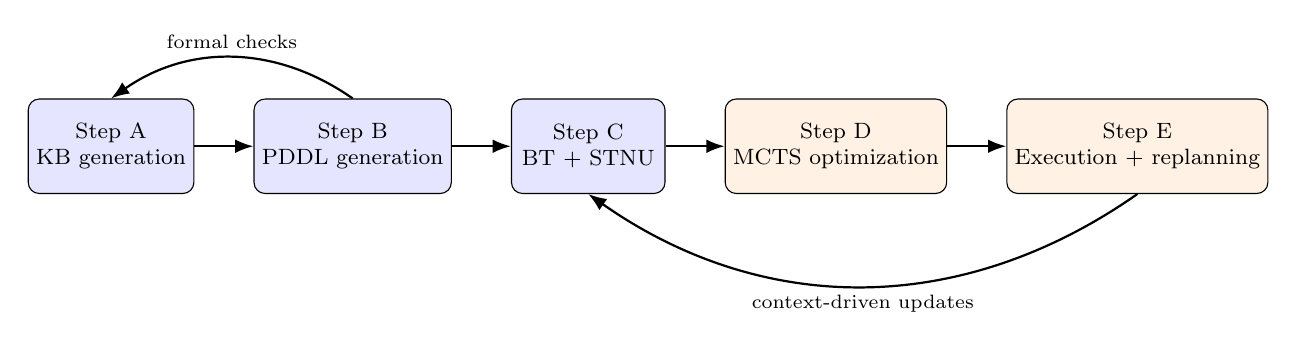
\begin{tikzpicture}[node distance=0.75cm, >=Latex, every node/.style={align=center}]
  \footnotesize
  \node[draw,rounded corners,fill=blue!10,minimum width=1.95cm,minimum height=1.2cm] (a) {Step A\\KB generation};
  \node[draw,rounded corners,fill=blue!10,minimum width=1.95cm,minimum height=1.2cm,right=of a] (b) {Step B\\PDDL generation};
  \node[draw,rounded corners,fill=blue!10,minimum width=1.95cm,minimum height=1.2cm,right=of b] (c) {Step C\\BT + STNU};
  \node[draw,rounded corners,fill=orange!10,minimum width=1.95cm,minimum height=1.2cm,right=of c] (d) {Step D\\MCTS optimization};
  \node[draw,rounded corners,fill=orange!10,minimum width=1.95cm,minimum height=1.2cm,right=of d] (e) {Step E\\Execution + replanning};
  \draw[->,thick] (a) -- (b); \draw[->,thick] (b) -- (c); \draw[->,thick] (c) -- (d); \draw[->,thick] (d) -- (e);
  \draw[->,thick,bend right=35] (b.north) to node[above,font=\scriptsize]{formal checks} (a.north);
  \draw[->,thick,bend left=35] (e.south) to node[below,font=\scriptsize]{context-driven updates} (c.south);
\end{tikzpicture}
\vspace{0.4em}
\begin{block}{Interpretation}
The methodology turns free-form language into a constrained planning pipeline that can be validated, optimized in a digital twin, and adapted at execution time.
\end{block}
%\refs{Source:\@proposal methodology Steps A-E.}

\end{frame}


\begin{frame}{Step A~-~Knowledge-Base Generation}

\begin{itemize}
  \item Generative AI is first used to create a \textbf{Knowledge Base (KB)} from a natural-language description of a class of processes.
  \item The KB captures \textbf{types, predicates and actions}, i.e., the formal domain description that planning needs.
  \item The process engineer validates the KB architecture; this is a \textbf{human-in-the-loop domain foundation} rather than blind end-to-end generation.
  \item Target evolution:\@from \textbf{TRL2 to TRL4} according to the proposal.
\end{itemize}
%\refs{Source:\@proposal Step A.}

\end{frame}


\begin{frame}{Step B~-~PDDL from Natural Language}

\begin{itemize}
  \item Once the domain is represented in the KB, natural-language task descriptions are converted into \textbf{PDDL descriptors} coherent with that domain.
  \item The proposal prefers this two-step strategy over direct end-to-end PDDL generation because a prior KB improves consistency and reduces hallucinated actions.
  \item Multi-agent generative AI and a \textbf{formal verification stage} iteratively refine the PDDL until it matches the stored domain definition.
  \item Target evolution:\@\textbf{TRL4 to TRL6} for the PDDL generation / verification chain.
\end{itemize}
%\refs{Source:\@proposal Step B and verification description.}

\end{frame}


\begin{frame}{Step C~-~Behavior Trees with Temporal Uncertainty}

\begin{itemize}
  \item The proposal converts verified PDDL into a \textbf{Behavior Tree} enriched by time-variance modelling.
  \item The enabling formalism is \textbf{STNU} (Simple Temporal Networks with Uncertainty), extending approaches based on standard STNs.
  \item The purpose is to capture duration variability without waiting for a perfect off-the-shelf temporal planner dealing with uncertainty.
  \item This is a core scientific novelty because it links symbolic planning to robust execution under variability.
\end{itemize}
%\refs{Source:\@proposal Step C.}

\end{frame}


\begin{frame}{Step D / E~-~Optimization, Execution and Replanning}

\small
\begin{itemize}
  \item The BT representation is optimized inside a \textbf{digital twin} using \textbf{Monte Carlo Tree Search} to identify the best policy under temporal variance.
  \item The result is then executed by a software module that runs the optimal BT and supports \textbf{online replanning}.
  \item The proposal distinguishes two runtime modes:
  \begin{itemize}
    \item an \textbf{anytime planning} module that continuously improves the plan while execution proceeds;
    \item a \textbf{heuristic restart} strategy for sudden, disruptive scene changes where feasibility matters more than optimality.
  \end{itemize}
\end{itemize}
%\refs{Source:\@proposal Step D/E and Activity 2 tasks.}

\end{frame}


\begin{frame}{Activity~2 (WP2)~-~Tasks, Timing and Outputs}

\small
\begin{tabularx}{\textwidth}{>{\bfseries}p{0.16\textwidth} p{0.16\textwidth} X}
\toprule
Task & Timing & Focus \\
\midrule
T2.1 & M7-M12 & Update the scientific plan according to the fast evolution of generative AI \\
T2.2 & M13-M24 & Lightweight LLM-based PDDL2 generation for robotic tasks \\
T2.3 & M18-M24 & PDDL2 to Behavior Tree generation with time-variance modelling \\
T2.4 & M22-M30 & Task and Motion Planning optimization in a digital twin environment \\
T2.5 & M28-M36 & Optimal BT execution and online replanning \\
T2.6 & M28-M36 & Integration inside MI.RA/Dexter low-code interface platform \\
T2.7 & M13-M36 & Continuous integration and versioning \\
T2.8 & M7-M12 & Benchmarking and evaluation setup \\
\bottomrule
\end{tabularx}
%\refs{Source:\@proposal Activity 2.}

\end{frame}


\begin{frame}{Module A~-~Expected Results, KPIs and TRL}

\small
\begin{tabularx}{\textwidth}{>{\bfseries}X c c}
\toprule
Indicator & KPI / target & TRL target \\
\midrule
Programming time reduction & 66\% reduction &~-~\\
Programming by non-pretrained worker & Demonstrated &~-~\\
KB correctness & 10 contexts evaluated & TRL2 $\rightarrow$ TRL4 \\
PDDL correctness & 100+ contexts & TRL2 $\rightarrow$ TRL4 \\
BT generation correctness & 100+ contexts & TRL4 $\rightarrow$ TRL6 \\
Optimal task planning evaluation & 100+ contexts & TRL2 $\rightarrow$ TRL4 \\
Fleet management & 3 mobile manipulators or 4 industrial arms &~-~\\
\bottomrule
\end{tabularx}
%\refs{Source:\@proposal Module A expected results and KPI subsections.}

\end{frame}


\section{Scientific Module B: Intelligent Sensing and Safe Motion Planning}

\begin{frame}{Module B~-~Scope}

\begin{itemize}
  \item Module~B couples \textbf{scene awareness} and \textbf{safe motion planning}. In the proposal, these are explicitly treated as inseparable.
  \item The challenge is collaborative robotics in dynamic workspaces where humans, mobile manipulators, and objects share the scene.
  \item The module spans sensing fusion, registration, semantic segmentation, symbolic-to-geometric grounding, offline planning, online replanning, and high-rate motion adaptation.
\end{itemize}
%\refs{Source:\@proposal ``Intelligent Sensing and Safe Motion Planning'' objectives.}

\end{frame}


\begin{frame}{Why Sensing and Planning Are Intertwined}

\begin{itemize}
  \item Task planning depends on knowing \textbf{which objects are present}, where they are, and how humans move in the workspace.
  \item Reactive motion adaptation only works if scene updates are timely and geometrically meaningful.
  \item Plan4ARI therefore aims at a \textbf{fully autonomous toolchain}:\@symbolic task descriptions should automatically become geometric and kinematic commands.
\end{itemize}
\begin{block}{Implication}
Scene understanding is not only for perception; it is a prerequisite for \textbf{safe and productive autonomy}. 
\end{block}
%\refs{Source:\@proposal objectives and methodology in Module B.}

\end{frame}


\begin{frame}{Sensor-Fusion Concept}

\centering
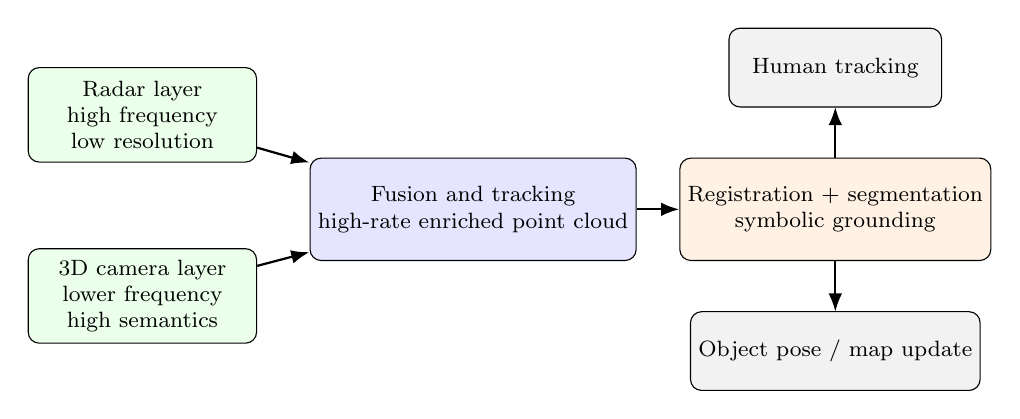
\begin{tikzpicture}[x=1cm,y=1cm,>=Latex,every node/.style={align=center}]
  \footnotesize
  \node[draw,rounded corners,fill=green!8,minimum width=2.9cm,minimum height=1.2cm] (radar) at (-4.2,1.4) {Radar layer\\high frequency\\low resolution};
  \node[draw,rounded corners,fill=green!8,minimum width=2.9cm,minimum height=1.2cm] (vision) at (-4.2,-0.9) {3D camera layer\\lower frequency\\high semantics};
  \node[draw,rounded corners,fill=blue!10,minimum width=3.4cm,minimum height=1.3cm] (fusion) at (0,0.2) {Fusion and tracking\\high-rate enriched point cloud};
  \node[draw,rounded corners,fill=orange!10,minimum width=3.4cm,minimum height=1.3cm] (scene) at (4.6,0.2) {Registration + segmentation\\symbolic grounding};
  \draw[->,thick] (radar) -- (fusion);
  \draw[->,thick] (vision) -- (fusion);
  \draw[->,thick] (fusion) -- (scene);
  \node[draw,rounded corners,fill=gray!10,minimum width=2.7cm,minimum height=1.0cm] at (4.6,2.0) {Human tracking};
  \node[draw,rounded corners,fill=gray!10,minimum width=2.7cm,minimum height=1.0cm] at (4.6,-1.6) {Object pose / map update};
  \draw[->,thick] (scene) -- (4.6,1.5);
  \draw[->,thick] (scene) -- (4.6,-1.1);
\end{tikzpicture}
\begin{block}{Proposed advantage}
Radar provides fast updates, while 3D vision provides accurate geometry and semantics; fusion should support safer and more responsive planning.
\end{block}
%\refs{Source:\@proposal methodology for sensing fusion and scene update.}

\end{frame}


\begin{frame}{State of the Art:\@Safety-Aware Motion Planning}

\small
\begin{itemize}
  \item Shared workspaces require more than collision-free motion:\@speed limitation and stops are triggered by safety modules implementing collaborative operations such as \textbf{SSM} and \textbf{PFL}.
  \item The proposal distinguishes \textbf{proactive} planning (avoiding expected interference beforehand) and \textbf{reactive} planning (modifying the path online).
  \item Existing methods have complementary weaknesses:\@proactive approaches degrade badly out of distribution; reactive approaches can lead to frequent stops and reduced efficiency.
  \item Plan4ARI explicitly aims to bridge them through \textbf{safety-aware replanning} coupled to human-aware costs.
\end{itemize}
%\refs{Source:\@proposal Module B state of the art discussion.}

\end{frame}


\begin{frame}{Planning Stack in Module B}

\begin{columns}[T,totalwidth=\textwidth]
\column{0.48\textwidth}
\begin{block}{Offline / asynchronous level}
\begin{itemize}
  \item global path computation,
  \item anytime replanning,
  \item digital-twin virtualization,
  \item Open IPC deployment.
\end{itemize}
\end{block}
\column{0.48\textwidth}
\begin{block}{Runtime / synchronous level}
\begin{itemize}
  \item scene-aware path repair,
  \item velocity modulation,
  \item visual-servo style synchronous planning,
  \item Core IPC MPC micro-interpolation.
\end{itemize}
\end{block}
\end{columns}
\begin{block}{Key design choice}
Planning is distributed across computation units according to latency and determinism requirements.
\end{block}
%\refs{Source:\@proposal objectives and methodology in Module B.}

\end{frame}


\begin{frame}{Informed Sampling and Replanning}

\begin{itemize}
  \item The module builds on sampling-based planning, especially \textbf{RRT-like} methods and informed sets.
  \item The proposal introduces a \textbf{mixed strategy}:\@global admissible informed sampling for asymptotic optimality, and local sampling around the current solution for fast improvement.
  \item The trade-off between exploration and exploitation is regulated adaptively using online rewards.
  \item A graph connecting pre-computed paths to the same goal supports efficient \textbf{multi-path replanning} when the current path is blocked.
\end{itemize}
%\refs{Source:\@proposal Module B methodology and Activity 4 task 4.2.}

\end{frame}


\begin{frame}{Safety-Aware Cost Functions}

\begin{itemize}
  \item A central proposal idea is that a path is not good enough if it is only collision-free; it must also reduce the intervention of the safety system.
  \item The planner therefore includes a \textbf{human-aware cost} based on ISO/TS~15066-inspired logic and uncertain human-state estimation.
  \item This extends prior work by the PI on safety-aware time-optimal motion planning and directly targets improved human-robot cooperation efficiency.
\end{itemize}
\begin{alertblock}{Expected benefit}
Fewer unnecessary slowdowns and stops, hence better productivity in collaborative scenarios.
\end{alertblock}
%\refs{Source:\@proposal methodology and cited Faroni et al. 2022 work.}

\end{frame}


\begin{frame}{MPC as Micro-Interpolator and Trajectory Filter}

\begin{itemize}
  \item The proposal uses \textbf{Model Predictive Control} not only as feedback control, but as a trajectory-generation and micro-interpolation engine.
  \item MPC predicts future robot states over a finite horizon, incorporates limits on joints, velocity, acceleration and workspace, and produces smooth feasible references.
  \item In Plan4ARI, MPC is meant to improve tracking under load, interface naturally with sensing (including visual servoing), and exploit residual degrees of freedom to reduce jerk or motor load.
\end{itemize}
%\refs{Source:\@proposal state of the art and methodology in Module B, plus Activity 4 task 4.3.}

\end{frame}


\begin{frame}{Activity~3 (Sensing for Context Awareness)}

\small
\begin{tabularx}{\textwidth}{>{\bfseries}p{0.16\textwidth} p{0.16\textwidth} X}
\toprule
Task & Timing & Focus \\
\midrule
T3.1 & M1-M6 & Update scientific plan for segmentation and pose estimation methodologies \\
T3.2 & M7-M9 & Market study and integration of radar sensors for scene monitoring \\
T3.3 & M10-M16 & Radar-camera fusion and tracking using multi-object methods \\
T3.4 & M17-M24 & Benchmarking and integration of semantic segmentation and 3D pose estimation methods \\
\bottomrule
\end{tabularx}
\vspace{0.4em}
\begin{block}{Expected output}
A sensing stack packaged as MI.RA/Dexter functional blocks and able to support tracking, registration and symbolic grounding.
\end{block}
%\refs{Source:\@proposal Activity 3.}

\end{frame}


\begin{frame}{Activity~4 (Local and Global Autonomous Motion Planning)}

\small
\begin{tabularx}{\textwidth}{>{\bfseries}p{0.16\textwidth} p{0.16\textwidth} X}
\toprule
Task & Timing & Focus \\
\midrule
T4.1 & M1-M6 & Update on motion-planning state of the art \\
T4.2 & M4-M24 & Informed sample-based optimal planning in dynamic environments \\
T4.3 & M4-M24 & MPC for adaptive micro-interpolation \\
T4.4 & M25-M30 & Integration in MI.RA/Dexter \\
T4.5 & M31-M36 & Integration of MPC inside COMAU Core IPC \\
T4.6 & M4-M36 & Continuous integration \\
T4.7 & M1-M6 & Benchmarking and evaluation design \\
\bottomrule
\end{tabularx}
%\refs{Source:\@proposal Activity 4.}

\end{frame}


\begin{frame}{Module B~-~Expected Results, KPIs and TRL}

\small
\begin{tabularx}{\textwidth}{>{\bfseries}X c c}
\toprule
Indicator & KPI / target & TRL target \\
\midrule
Motion-plan generation & Fully autonomous joint and Cartesian plans &~-~\\
Interaction execution time & 30\% reduction vs.\ state-of-the-art planners &~-~\\
Computation time benchmark & Mean over 100+ contexts & TRL5 $\rightarrow$ TRL7 \\
Scene-update / registration accuracy & About 20\% better than standard 3D-vision registration & TRL4 $\rightarrow$ TRL6 \\
Tracking performance under dynamics load & About 50\% improvement & TRL5 $\rightarrow$ TRL7 \\
Safe velocity adaptation & Demonstrated under varying working conditions &~-~\\
\bottomrule
\end{tabularx}
%\refs{Source:\@proposal Module B expected results and KPI subsections.}

\end{frame}


\section{Scientific Module C: Neural Motion Control}

\begin{frame}{Module C~-~Motivation}

\begin{itemize}
  \item In the proposal, the inner layer of ARI is the \textbf{high-rate real-time motion controller}.
  \item Conventional industrial control relies on accurate models, full-state observers and careful tuning; this is powerful but expensive to deploy and difficult in the presence of elasticity and uncertainty.
  \item Plan4ARI seeks a new generation of \textbf{adaptive neural controllers} that can run on industrial PCs while preserving robustness and safety.
\end{itemize}
%\refs{Source:\@proposal ``Advanced Robot Motion Controlling through Machine Learning Methods~-~Objectives''.}

\end{frame}


\begin{frame}{State of the Art and Limits}

\small
\begin{itemize}
  \item The proposal reviews several observer families:\@\textbf{UKF}, \textbf{sliding-mode observers}, and \textbf{high-gain observers}. Each has strengths, but compromises appear in computational burden, noise sensitivity, or robustness.
  \item Neural control is appealing because it naturally handles nonlinear dynamics, disturbances, and rich sensing inputs.
  \item The remaining barriers are \textbf{computational burden}, \textbf{robustness demonstration}, and integration with sensing and industrial real-time constraints.
\end{itemize}
%\refs{Source:\@proposal Module C state of the art.}

\end{frame}


\begin{frame}{Control Concept:\@Prescribed Performance + Learning}

\begin{itemize}
  \item The proposal combines \textbf{Prescribed Performance Control (PPC)} with adaptive learning, specifically \textbf{RBF neural networks}.
  \item PPC predefines acceptable transient and steady-state behavior; learning then estimates and compensates unknown dynamics while respecting those envelopes.
  \item The controller is designed to cope with \textbf{modelling uncertainty, actuator failures, motion constraints, and joint elasticity}. 
\end{itemize}
%\refs{Source:\@proposal Module C objectives and methodology.}

\end{frame}


\begin{frame}{Neural Control Methodology}

\small
\begin{enumerate}
  \item Define a dynamic learning scheme for industrial manipulators including lumped elastic effects.
  \item Transform the constrained tracking problem into an unconstrained stabilization variable through an \textbf{error transformation}.
  \item Use filtered errors and adaptive neural control to force tracking errors to a small neighborhood while satisfying prescribed performance.
  \item Transform the closed-loop dynamics into an LTV structure with small perturbations, enabling accurate convergence of neural weights.
  \item Store the converged weights so that learned knowledge can be \textbf{reused} on similar tasks.
\end{enumerate}
%\refs{Source:\@proposal Module C methodology.}

\end{frame}


\begin{frame}{Why the Proposed Controller Matters}

\begin{columns}[T,totalwidth=\textwidth]
\column{0.52\textwidth}
\begin{block}{Claimed advantages}
\begin{itemize}
  \item easy integration of compliance modelling,
  \item no need for a full-state observer,
  \item MIMO design without matrix inversion,
  \item straightforward integrator modelling,
  \item limited computation time.
\end{itemize}
\end{block}
\column{0.44\textwidth}
\begin{block}{Industrial consequence}
The controller should reduce tuning effort, shorten deployment time, and improve high-dynamics tracking performance without violating industrial real-time constraints.
\end{block}
\end{columns}
%\refs{Source:\@proposal Module C methodology and expected results.}

\end{frame}


\begin{frame}{Activity~5 (Neural Robust Motion Control)}

\small
\begin{tabularx}{\textwidth}{>{\bfseries}p{0.16\textwidth} p{0.16\textwidth} X}
\toprule
Task & Timing & Focus \\
\midrule
T5.1 & M1-M6 & Scientific-plan update for control methodologies \\
T5.2 & M4-M30 & Design and proof of the neural controller with prescribed-performance constraints \\
T5.3 & M12-M36 & Integration in COMAU Open IPC / platform wrapper \\
T5.4 & M4-M36 & Continuous integration \\
T5.5 & M1-M6 & Benchmarking and evaluation setup \\
\bottomrule
\end{tabularx}
%\refs{Source:\@proposal Activity 5.}

\end{frame}


\begin{frame}{Module C~-~Expected Results, KPIs and TRL}

\small
\begin{tabularx}{\textwidth}{>{\bfseries}X c c}
\toprule
Indicator & KPI / target & TRL target \\
\midrule
Auto-tuning of dynamics/control parameters & Demonstrated &~-~\\
Mean tracking error & About 10\% reduction & TRL5 $\rightarrow$ TRL7 \\
Overshoot under high dynamics & About 30\% reduction & TRL5 $\rightarrow$ TRL7 \\
Computation time stress tests & Mean over 200+ contexts & TRL2 $\rightarrow$ TRL5 \\
Deployment time of a running controller & About 50\% reduction vs current COMAU time & TRL4 $\rightarrow$ TRL6 \\
\bottomrule
\end{tabularx}
%\refs{Source:\@proposal Module C expected results and KPI subsections.}

\end{frame}


\section{Scientific Module D: Trustworthiness and Human-Centric Optimization}

\begin{frame}{Module D~-~Why Trustworthiness is a Technical Variable}

\begin{itemize}
  \item The proposal treats trustworthiness not as an afterthought, but as a component of the robotic architecture.
  \item Adoption barriers are cultural as well as technical:\@workers must trust hardware, software, safety logic and the quality of robot cooperation.
  \item The project therefore develops both \textbf{subjective} and \textbf{objective} measures of human acceptance and interaction quality.
\end{itemize}
%\refs{Source:\@proposal ``Trustworthiness and Human-Centric Optimization~-~Objectives''.}

\end{frame}


\begin{frame}{Trustworthiness Methodology}

\small
\begin{itemize}
  \item Design new subject-evaluation forms specific to \textbf{AI-powered industrial HRC}.
  \item Validate them statistically on an initial population and then deploy them on a larger sample.
  \item Develop objective, ideally non-intrusive metrics based on interaction quality during operation.
  \item Map objective data and perceived trust to the project \textbf{Knowledge Base}, so that human factors can influence decision support and risk assessment.
\end{itemize}
%\refs{Source:\@proposal trustworthiness methodology.}

\end{frame}


\begin{frame}{What Is Measured?}

\small
\begin{tabularx}{\textwidth}{>{\bfseries}p{0.28\textwidth} X}
\toprule
Dimension & Examples in the proposal \\
\midrule
Perceived safety & Trust in not being physically damaged; trust in safety software \\
Task quality & Whether robot and operator effectively accomplish the job \\
Role / agency & Whether the operator feels leading, equal to, or driven by the cobot \\
Stress / workload & Mental and physical stress before, during and after shifts \\
Human-robot relationship & Relevance of the cobot identity, tool vs colleague perception \\
Dynamic interaction quality & Intention recognition, space negotiation, unexpected breaks in cooperation \\
\bottomrule
\end{tabularx}
%\refs{Source:\@proposal Activity 6 task T6.1 and trustworthiness objectives.}

\end{frame}


\begin{frame}{Activity~6 (Human-Robot Trustworthiness Evaluation and Assessment)}

\small
\begin{tabularx}{\textwidth}{>{\bfseries}p{0.16\textwidth} p{0.16\textwidth} X}
\toprule
Task & Timing & Focus \\
\midrule
T6.1 & M7-M9 & Design of the questionnaire and topic refinement with operators \\
T6.2 & M10-M16 & Validation campaign with at least 50 workers \\
T6.3 & M17-M24 & Statistical refinement and final questionnaire deployment \\
T6.4 & M24-M36 & Evaluation campaign and dataset creation with 100+ workers \\
\bottomrule
\end{tabularx}
%\refs{Source:\@proposal Activity 6.}

\end{frame}


\begin{frame}{Module D~-~Expected Results, KPIs and TRL}

\scriptsize
\begin{tabularx}{\textwidth}{>{\bfseries}X c c}
\toprule
Indicator & KPI / target & TRL target \\
\midrule
Subjective trustworthiness metrics & 100+ workers; open dataset statistics & TRL9 (existing generic practice) $\rightarrow$ tailored TRL5 \\
Objective trustworthiness metrics & 10+ consortium workers; open statistics & TRL3 $\rightarrow$ TRL4 \\
Continuous monitoring & Data-driven and context-aware dynamic measures &~-~\\
Integration into control framework & Human-centric optimization and KB update &~-~\\
\bottomrule
\end{tabularx}
%\refs{Source:\@proposal Module D expected results and KPI subsections.}

\end{frame}


\section{Project Plan, Activities and Management}

\begin{frame}{Project Logic Across Activities}

\centering
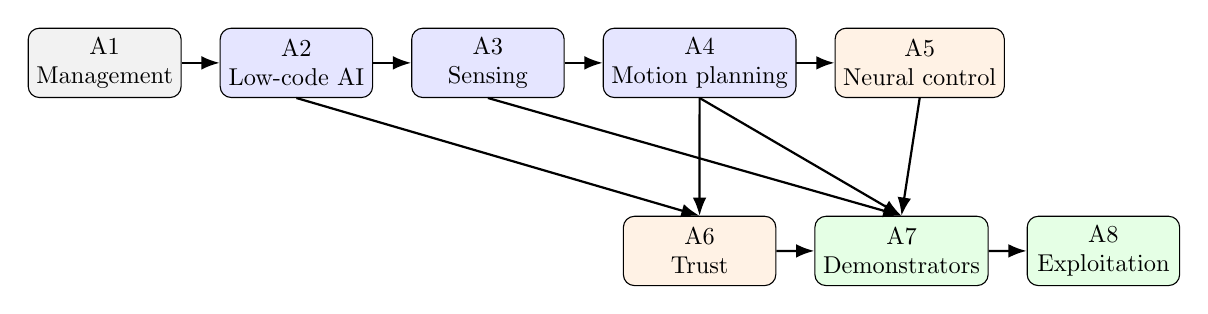
\begin{tikzpicture}[node distance=0.55cm, >=Latex, every node/.style={align=center}, scale=0.88, transform shape]
\node[draw,rounded corners,fill=gray!10,minimum width=2cm,minimum height=1cm] (a1) {A1\\Management};
\node[draw,rounded corners,fill=blue!10,minimum width=2.2cm,minimum height=1cm,right=of a1] (a2) {A2\\Low-code AI};
\node[draw,rounded corners,fill=blue!10,minimum width=2.2cm,minimum height=1cm,right=of a2] (a3) {A3\\Sensing};
\node[draw,rounded corners,fill=blue!10,minimum width=2.2cm,minimum height=1cm,right=of a3] (a4) {A4\\Motion planning};
\node[draw,rounded corners,fill=orange!10,minimum width=2.2cm,minimum height=1cm,right=of a4] (a5) {A5\\Neural control};
\node[draw,rounded corners,fill=orange!10,minimum width=2.2cm,minimum height=1cm,below=1.7cm of a4] (a6) {A6\\Trust};
\node[draw,rounded corners,fill=green!10,minimum width=2.2cm,minimum height=1cm,right=of a6] (a7) {A7\\Demonstrators};
\node[draw,rounded corners,fill=green!10,minimum width=2.2cm,minimum height=1cm,right=of a7] (a8) {A8\\Exploitation};
\draw[->,thick] (a1) -- (a2); \draw[->,thick] (a2) -- (a3); \draw[->,thick] (a3) -- (a4); \draw[->,thick] (a4) -- (a5);
\draw[->,thick] (a2.south) -- (a6.north); \draw[->,thick] (a4.south) -- (a6.north);
\draw[->,thick] (a3.south) -- (a7.north); \draw[->,thick] (a4.south) -- (a7.north); \draw[->,thick] (a5.south) -- (a7.north);
\draw[->,thick] (a6.east) -- (a7.west);
\draw[->,thick] (a7) -- (a8);
\end{tikzpicture}
\begin{block}{Reading}
Management and data governance support all activities. Activities 2--5 deliver the technical stack, Activity~6 validates human acceptance, Activity~7 integrates the final demonstrators, and Activity~8 drives dissemination and exploitation.
\end{block}
%\refs{Source:\@proposal activity list and project organization.}

\end{frame}


\begin{frame}{Activity 1~-~Scientific, Technical and Project Management}

\small
\begin{itemize}
  \item \textbf{Objective:} guarantee that technical, financial, administrative and coordination aspects remain aligned with scientific objectives over 48 months.
  \item \textbf{Task 1.1:} general management, project templates, reporting procedures, internal communication, gender-equality attention.
  \item \textbf{Task 1.2:} financial management and audit preparation.
  \item \textbf{Task 1.3:} technical and risk coordination, deliverable quality monitoring, data-management-plan updates, contingency actions.
  \item \textbf{Task 1.4:} research data management with informed consent, anonymization, GDPR compliance and ethics alignment.
  \item \textbf{Task 1.5:} advisory board creation within the first 6 months.
\end{itemize}
%\refs{Source:\@proposal Activity 1.}

\end{frame}


\begin{frame}{Activity 2~-~Low-Code Programming with Generative and Deliberative AI}

\small
\begin{itemize}
  \item \textbf{Objective:} reduce programming time and move programming authority from robot experts to process experts.
  \item Scientific work spans the complete chain:\@state-of-the-art update, PDDL generation with lightweight LLMs, BT/STNU conversion, MCTS optimization, online replanning, and MI.RA/Dexter integration.
  \item Continuous integration and early benchmarking are included as dedicated tasks, which is important for industrial software maturity.
  \item This activity is the main symbolic/planning entry point for the whole architecture.
\end{itemize}
%\refs{Source:\@proposal Activity 2.}

\end{frame}


\begin{frame}{Activity 3~-~Sensing for Context Awareness}

\small
\begin{itemize}
  \item \textbf{Objective:} monitor the robot workspace with radar and 3D vision, and provide robust operator tracking and object understanding.
  \item The work is staged:\@methodology update, radar acquisition/integration, radar-camera data fusion, benchmarking of segmentation/pose-estimation pipelines.
  \item The final output is a set of functional sensing blocks embedded in MI.RA/Dexter and connected to motion planning.
\end{itemize}
%\refs{Source:\@proposal Activity 3.}

\end{frame}


\begin{frame}{Activity 4~-~Local and Global Autonomous Motion Planning}

\small
\begin{itemize}
  \item \textbf{Objective:} develop planners for teams of manipulators in collaborative dynamic environments.
  \item The activity combines algorithmic research (informed sample-based planning and MPC micro-interpolation) with direct integration in the COMAU stack.
  \item The deliverable logic clearly separates algorithm prototyping from the more delicate integration of MPC in the Core IPC.\@
  \item Continuous integration and benchmarking are explicit, which should help maintain reproducibility and software quality.
\end{itemize}
%\refs{Source:\@proposal Activity 4.}

\end{frame}


\begin{frame}{Activity 5~-~Neural Robust Motion Control}

\small
\begin{itemize}
  \item \textbf{Objective:} push robot low-level control beyond industrial SOTA through neural control algorithms with prescribed-performance constraints.
  \item Technical work includes modeling of lumped elasticity, controller design and proof, simulation in COMAU-developed environments, and later C++ implementation.
  \item Integration uses containerized logic and the existing Open IPC / platform interfaces to accelerate industrial deployment while preserving safety engineering discipline.
\end{itemize}
%\refs{Source:\@proposal Activity 5.}

\end{frame}


\begin{frame}{Activity 6~-~Human-Robot Trustworthiness Evaluation and Assessment}

\small
\begin{itemize}
  \item \textbf{Objective:} create a tool that helps manufacturers assess workers' engagement and acceptance when operating with AI-powered collaborative robots.
  \item The activity intentionally follows a staged psychometric process:\@initial questionnaire design, validation with 50 workers, refinement, and final deployment at 100+ workers.
  \item This is crucial because the project wants trust metrics that are not generic but \textbf{specific to industrial AI-powered HRC}. 
\end{itemize}
%\refs{Source:\@proposal Activity 6.}

\end{frame}


\begin{frame}{Activity 7~-~Targeted Demonstrators}

\small
\begin{itemize}
  \item \textbf{Objective:} validate the integrated Plan4ARI stack on three sector-specific demonstrators provided by COMAU.\@
  \item The demonstrators are not add-ons; they are the project-level integration test for low-code task generation, sensing, planning, control and trustworthiness assessment.
  \item The three scenarios are:\@warehouse picking, remanufacturing, and welding in large ships.
\end{itemize}
%\refs{Source:\@proposal Activity 7.}

\end{frame}


\begin{frame}{Activity 8~-~Communication, Dissemination and Exploitation}

\small
\begin{itemize}
  \item \textbf{Objective:} maintain communication channels, disseminate scientific and industrial results, and structure exploitation plans and business cases.
  \item The activity includes website, public materials, digital media, workshops, publications, fairs, and a maintained exploitation culture.
  \item It also covers market analysis, foreground management, patent surveys, and exploitation planning.
\end{itemize}
%\refs{Source:\@proposal Activity 8.}

\end{frame}


\begin{frame}{Roles of PI, Research Organization and Host}

\small
\begin{tabularx}{\textwidth}{>{\bfseries}p{0.22\textwidth} X}
\toprule
Actor & Role in the proposal \\
\midrule
PI & Scientific coordination, methodology design, continuous technical steering, weekly touch points with teams and COMAU responsibles \\
Research Organization (CNR) & Fundamental and industrial research, methodology definition, prototyping, scientific implementation, benchmarking support \\
Host Institution (COMAU) & Platform access, industrial development teams, sensing and low-level control integration, innovation teams, demonstrator provision and evaluation \\
\bottomrule
\end{tabularx}
%\refs{Source:\@role descriptions repeated in Modules A-D and institution sections.}

\end{frame}


\begin{frame}{Module-Level Resource Allocation Mentioned in the Proposal}

\small
\begin{tabularx}{\textwidth}{>{\bfseries}p{0.25\textwidth} c c X}
\toprule
Module & Research Org. & Host & Comment \\
\midrule
Module A~-~Low-code & $>$30\% & about 35\% & Strong co-development with MI.RA/Dexter teams \\
Module B~-~Sensing / motion planning & about 35\% & about 35\% & Shared effort across perception, planner integration and Core IPC work \\
Module C~-~Neural control & about 25\% & about 27.5\% & Significant industrial integration and digital-twin support \\
Module D~-~Trustworthiness & about 10\% & about 2.5\% & Mainly research-led with innovation-department support \\
\bottomrule
\end{tabularx}
\begin{block}{Note}
The proposal includes a budget-plan figure and refers to co-financing details in Allegato~B;\@the table above summarizes the explicit percentage statements available in the text.
\end{block}
%\refs{Source:\@roles and budget mentions in module sections and budget plan section.}

\end{frame}


\begin{frame}{Deliverables (1/2)}

\scriptsize
\begin{tabularx}{\textwidth}{>{\bfseries}p{0.12\textwidth} X p{0.10\textwidth}}
\toprule
ID & Deliverable & Due \\
\midrule
D1.1 & Management Report & M12 \\
D1.2 & Management Report & M24 \\
D1.3 & Management Report & M36 \\
D1.4 & Management Report & M48 \\
D2.1 & Scientific Plan and First Running Mockup of the Low-Coding Module & M12 \\
D2.2 & First Running Time-Variance Aware Planner in MI.RA/Dexter & M24 \\
D2.3 & Optimal Task and Motion Planning with online replanning module & M36 \\
D3.1 & Scientific Plan and First Running Mockup for the sensing module & M12 \\
D3.2 & Sensing Methodologies and First Prototypes Release & M24 \\
D3.3 & Sensing Modules integrated in the COMAU IPC & M36 \\
D4.1 & Scientific Plan and First Mockup of the Motion Planning Modules & M12 \\
D4.2 & Motion Planners Modules Prototypes & M24 \\
\bottomrule
\end{tabularx}
%\refs{Source:\@proposal ``List of Deliverables''.}

\end{frame}


\begin{frame}{Deliverables (2/2)}

\scriptsize
\begin{tabularx}{\textwidth}{>{\bfseries}p{0.12\textwidth} X p{0.10\textwidth}}
\toprule
ID & Deliverable & Due \\
\midrule
D4.3 & Motion Planners Modules Prototypes integrated in the COMAU IPC & M36 \\
D5.1 & Scientific Plan and First Mockup of the Neural Control Architecture & M12 \\
D5.2 & First Release of the Neural Controller Prototype & M24 \\
D5.3 & Neural Control Architecture integrated in the COMAU IPC & M36 \\
D6.1 & Scientific Plan and First Questionnaire Release & M12 \\
D6.2 & Second Questionnaire Release & M24 \\
D6.3 & Campaign Evaluation Report & M36 \\
D7.1 & Demonstrators &~-~\\
D8.1 & Exploitation, Communication, Dissemination Report & M12 \\
D8.2 & Exploitation, Communication, Dissemination Report & M24 \\
D8.3 & Exploitation, Communication, Dissemination Report & M36 \\
\bottomrule
\end{tabularx}
%\refs{Source:\@proposal ``List of Deliverables''. Note:\@the proposal appears to repeat D5.2 numbering; here D5.3 is used for the M36 integration deliverable to keep the deck coherent.}

\end{frame}


\begin{frame}{Milestones and Means of Verification}

\small
\begin{tabularx}{\textwidth}{>{\bfseries}p{0.12\textwidth} >{\bfseries}p{0.10\textwidth} X}
\toprule
Milestone & Due & Means of verification \\
\midrule
MS1 & M12 & D1.1, D2.1, D3.1, D4.1, D5.1, D6.1, D7.1, D8.1 \\
MS2 & M24 & D1.2, D2.2, D3.2, D4.2, D5.2, D6.2, D7.2, D8.2 \\
MS3 & M36 & D1.3, D2.3, D3.3, D4.3, D5.3, D6.3, D7.3, D8.3 \\
MS4 & M48 & D1.4 and final integrated demonstrator / closure set indicated in the proposal \\
\bottomrule
\end{tabularx}
\begin{block}{Observation}
Milestones are structured as integration gates coupling management, technical modules, validation and dissemination.
\end{block}
%\refs{Source:\@proposal ``List of Milestones''; note the proposal contains some numbering inconsistencies in the milestone verification lists.}

\end{frame}


\begin{frame}{Global GANTT}

\scriptsize
\begin{center}
\begin{ganttchart}[
  x unit=0.16cm,
  y unit chart=0.36cm,
  hgrid,
  vgrid,
  milestone label font=\scriptsize,
  bar label font=\scriptsize,
  title label font=\scriptsize,
  title height=1,
  bar/.append style={fill=planblue!60},
  group/.append style={fill=planorange!60}
]{1}{48}
\gantttitlelist{1,...,48}{1} \\
\ganttbar{A1 Management}{1}{48} \\
\ganttbar{A2 Low-code AI}{1}{36} \\
\ganttbar{A3 Sensing}{1}{24} \\
\ganttbar{A4 Motion planning}{1}{36} \\
\ganttbar{A5 Neural control}{1}{36} \\
\ganttbar{A6 Trust evaluation}{7}{42} \\
\ganttbar{A7 Demonstrators}{36}{48} \\
\ganttbar{A8 Dissemination / exploitation}{1}{48} \\
\ganttmilestone{MS1}{12} \ganttmilestone{MS2}{24} \ganttmilestone{MS3}{36} \ganttmilestone{MS4}{48}
\end{ganttchart}
\end{center}
%\refs{Source:\@proposal GANTT figure and activity timing table.}

\end{frame}


\begin{frame}{Detailed Critical Path Reading}

\begin{itemize}
  \item \textbf{Months 1--12:} scientific-plan updates, benchmarking setup, and first mockups in Modules A-D build the technical baseline for MS1.
  \item \textbf{Months 13--24:} low-code planning chain, sensing fusion, informed planning, and neural-controller design mature to prototype level and define MS2.
  \item \textbf{Months 25--36:} industrial integration in MI.RA/Dexter and COMAU IPC, online replanning, and trust-evaluation campaigns culminate in MS3.
  \item \textbf{Months 36--48:} targeted demonstrators and final exploitation close the project and anchor MS4.
\end{itemize}
%\refs{Source:\@proposal activity schedule, deliverables and milestones.}

\end{frame}


\section{Demonstrators, Impact and Risk}

\begin{frame}{Targeted Demonstrators~-~Overview}

\small
\begin{tabularx}{\textwidth}{>{\bfseries}p{0.18\textwidth} X X}
\toprule
Demo & Use case & Why it matters \\
\midrule
D7.1 & Warehouse picking of heterogeneous objects & Tests natural-language tasking, object grounding, and collaborative intralogistics \\
D7.2 & Remanufacturing and disassembly of mechanical components & Tests planning, interaction control, force-sensitive behavior and rescheduling \\
D7.3 & Welding of plates in large ship structures with mobile manipulators & Tests operation in harsh, cluttered, safety-critical environments with limited ability to deviate from nominal paths \\
\bottomrule
\end{tabularx}
%\refs{Source:\@proposal Activity 7.}

\end{frame}


\begin{frame}{Demonstrator 1~-~Warehouse Picking}

\begin{itemize}
  \item The robot must manipulate a wide variety of objects, including soft or non-standard items, in a dynamic warehouse without rigid layouts.
  \item The operator may issue commands such as \textit{``Pick the red t-shirt in box A and put it in box B''}.
  \item The system must translate language into robot programmes, allocate tasks, plan trajectories, continuously monitor the scene, and replan under human presence.
  \item This demonstrator heavily exercises \textbf{KB creation, semantic segmentation, robot localization, and online motion planning}. 
\end{itemize}
%\refs{Source:\@proposal Activity 7 task 7.1.}

\end{frame}


\begin{frame}{Demonstrator 2~-~Remanufacturing}

\begin{itemize}
  \item Focuses on disassembly/remanufacturing of mechanical components, where flexible intervention and sustainable manufacturing are key.
  \item Human operators guide the robot through natural language, while the integrated stack generates optimized task and motion plans.
  \item The scenario stresses interaction-aware replanning, low-level control performance, and robot-environment force interaction.
  \item It is the most direct demonstration of the synergy between \textbf{task planning, sensing, MPC, and neural control}. 
\end{itemize}
%\refs{Source:\@proposal Activity 7 task 7.2.}

\end{frame}


\begin{frame}{Demonstrator 3~-~Ship Welding}

\begin{itemize}
  \item Targets a very harsh industrial domain where welding is still largely manual, harmful and difficult to fence.
  \item Mobile manipulators must work in huge cluttered structures where operators remain nearby.
  \item Unlike generic path replanning tasks, welding often forbids significant deviation from the nominal path:\@the system must stop safely and resume correctly.
  \item This demonstrator is therefore the most demanding test of \textbf{localization, sensing fusion, runtime safety, and human acceptance}. 
\end{itemize}
%\refs{Source:\@proposal Activity 7 task 7.3.}

\end{frame}


\begin{frame}{Expected Scientific and Industrial Impact}

\begin{itemize}
  \item Scientifically, the project proposes a \textbf{systematic framework for cognitive industrial robotics}, rather than isolated algorithms.
  \item Industrially, it aims to show that AI can be integrated into standard industrial toolchains to reduce programming effort, improve throughput, reduce errors and improve ergonomics.
  \item The proposal links its ambition to AI in manufacturing, mobile manipulation and collaborative robotics, stressing European competitiveness and SME accessibility.
\end{itemize}
%\refs{Source:\@proposal ``Innovativeness and originality'' and ``Expected impact''.}

\end{frame}


\begin{frame}{Socio-Economic Effect and Job Quality}

\begin{itemize}
  \item The proposal sets an explicit target of \textbf{15\% increase in the OECD Job Quality Index} through safer and more ergonomic work environments.
  \item Expected benefits include reduced accident exposure, lower operator stress, improved information delivery to workers, and better transparency in collaborative workspaces.
  \item This is one of the strongest distinguishing factors of the project:\@productivity gains are tied to \textbf{human-centric acceptance and workplace quality}. 
\end{itemize}
%\refs{Source:\@proposal ``Socio-economic Impact''.}

\end{frame}


\begin{frame}{Requirements, Risks and Mitigation}

\small
\begin{tabularx}{\textwidth}{>{\bfseries}p{0.19\textwidth} X X}
\toprule
Risk factor & Proposal concern & Mitigation logic \\
\midrule
Market challenger & New entrants may challenge specific AI controllers & Modular open architecture and service-oriented exploitation \\
Performance & Multi-layer architecture may reduce overall performance & Fine-tuning, solver replacement, suboptimal feasible modes \\
Scalability & Complex dependencies may hinder reuse & Abstract interfaces and minimized dependencies \\
Computational burden & Several modules may become heavy & Relax optimality to preserve feasibility \\
Legal framework & Regulation changes and EU AI Act concerns on biometrics/emotions & GDPR-like anonymization, online-only methods, ethics review \\
Adoption & Users may reject AI-driven robots & Trust metrics and clear communication strategy \\
\bottomrule
\end{tabularx}
%\refs{Source:\@proposal ``Requirements, potential barriers, and mitigation measures''.}

\end{frame}


\begin{frame}{Conclusion}

\begin{block}{Plan4ARI in one sentence}
A 48-month program to turn industrial robots into \textbf{trustworthy cognitive agents} by integrating natural language interaction, verified planning, scene-aware motion planning, adaptive real-time control and human-centric trust evaluation.
\end{block}
\begin{itemize}
  \item Strong industrial anchor through COMAU, with access to real platforms, demonstrators and industrial expertise.
  \item Strong scientific foundation through CNR-STIIMA, with a clear focus on algorithmic development and integration.
  \item Clear integration path through eight activities, demonstrators, KPIs, milestones and deliverables.
  \item High relevance for Industry~5.0, advanced manufacturing and collaborative robotics.
\end{itemize}
%\refs{Source:\@full proposal synthesis.}

\end{frame}

\end{document}
